

\documentclass[journal]{IEEEtran}

\usepackage{cite}
\usepackage{amsmath}
\interdisplaylinepenalty=2500
\usepackage{algorithm}
\usepackage[noend]{algpseudocode}
\usepackage{array}
\usepackage{graphicx}
\usepackage{float}

% correct bad hyphenation here
\hyphenation{op-tical net-works semi-conduc-tor}


\begin{document}
\title{Detection of circle grid patterns \\ for camera calibration}

\author{Wilbert~Pumacay,~\textit{Catholic University San Pablo},~wilbert.pumacay@ucsp.edu.pe\\
        Gerson~Vizcarra,~\textit{Catholic University San Pablo},~gerson.vizcarra@ucsp.edu.pe}

% make the title area
\maketitle

\begin{abstract}
Camera calibration is an step in several applications, like augmented reality. To do calibration properly using current calibration methods we need to get features we can related in both 2D camera space and 3D world space to estimate the camera parameters that give this mapping. In this context, the use of grid patterns help by giving us the features we need, being the components in the pattern which we must detect in every frame in video.
\\
\\
In this paper we study some techniques to make this process of feature extraction by implementing a pipeline that gets these features by combining various techniques from classical image processing.
\end{abstract}

\begin{IEEEkeywords}
Camera calibration, calibration pattern, circle grid, image processing.
\end{IEEEkeywords}


\section{Introduction}

\IEEEPARstart{T}{he} camera calibration problem consists of finding 11 parameters that describe the mapping between 2D camera space and 3D world space. Six parameters, called extrinsic, come from an homogeneous transform, giving 6 parameters ( rotation and translation around the axes ). The other 5 parameters, called intrinsic, define some internal properties of the camera. This can be expressed in the following transformation equation :

\begin{equation}
  \begin{bmatrix}
    \mu \\
    \nu \\
      1 
  \end{bmatrix} = 
  \begin{bmatrix}
    \alpha & \gamma & \mu_{0} \\
       0   & \beta  & \nu_{0} \\
       0   &    0   &    1
  \end{bmatrix} 
  \begin{bmatrix}
    r_{x_{1}} & r_{y_{1}} & r_{z_{1}} & t_{x}\\
    r_{x_{2}} & r_{y_{2}} & r_{z_{2}} & t_{y}\\
    r_{x_{3}} & r_{y_{3}} & r_{z_{3}} & t_{z}
  \end{bmatrix} 
  \begin{bmatrix}
    x \\
    y \\
    z \\
    1
  \end{bmatrix}
%
\end{equation}

To find these parameters, camera calibration methods make use of correspondances between 2D and 3D spaces in order to fit the parameters that best describe this mapping. We achieve this by minimizing the following function :

\begin{equation}
  \sum^{m}_{i} \sum^{n}_{j} \Vert TP^{ij}_{3D} - P^{ij}_{2D} \Vert^{2}
\end{equation}

Where we are trying to minimize the difference between the expected projection and the actual projection over some set of features.The key idea is that supplying sufficient features that have a correct mapping, we can get the 11 parameters needed that minimize this function. So, a key part is the detection of these features.
\\
\\
In equation $2$ we are looping through a set of features $n$ that are found in each frame of a video of $m$ frames, so, we basically need to detect some feature points in each frame of video, which is what we focus in this paper.

\section{About the method}
To extract these features from every frame of video we implemented the following pipeline using image processing primitives.

\begin{figure}[H]
\centering
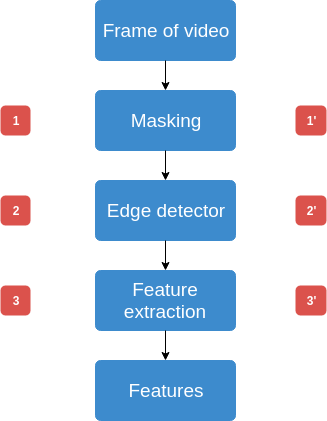
\includegraphics[width=2.5in]{_img/algorithm_overview.png}
\caption{Pattern detection pipeline.}
\end{figure}

\subsection{Masking}
This step is in charge of isolating the pattern by using threhsolding operations. We used two approaches :
\\
\\
The first approach is to segment the desired areas by using ranges in a color space. We tried HSV and RGB color spaces, but the YCrCb was the one that gave us better results. There, we could extract more easily the pattern because of its white colour.
\\
\\
In order to compensate for the ilumination changes, we \textbf{equalized} the $Y$ channel and insert it back into the image to check for ranges. Once we have the binary image, we apply the \textbf{opening} morphological operator to get rid of noise in the mask. After that, we just apply a \textbf{bitwise and} operation with the grayscale image for further edge detection using Canny's algorithm.
%%
\begin{algorithm}
\caption{Masking 1}
\begin{algorithmic}[1]
\State $\textit{Set up thresholding ranges}$
\State $mask   = \textit{ColorSpaceThresholding}(inputImage)$
\State $mask   = \textit{MorphologicalOpening}(mask, kernelSize)$
\State $masked = \textit{BitwiseAnd}( \textit{rgb2gray}( inputImage ), mask )$\\
\Return $masked$
\end{algorithmic}
\end{algorithm}
\\
\\
The second approach consists on creating a mask from the grayscale transformed image applying \textbf{Adaptive Thresholding algorithm}, this algorithm relies on Integral Image technique especified in \cite{IntegralImageThresholding}.
\\
\\
Before apply this transformation we tried to transform the color frame to LAB color space and equalize L channel in order to control luminosity changes across the video frames, but the main issue in this heuristic was that the transformation trends to emphasize other regions with very low luminance like desk reflection on a video, and this produces noisy results.
\\
\\
%% TODO: Gerson
\begin{algorithm}
\caption{Masking 2}
\label{alg:mask2}
\begin{algorithmic}[1]
\State $\textit{Set up thresholding parameters}$
\State $mask   = \textit{rgb2gray}( inputImage )$
\State $mask   = \textit{AdaptiveThreshold}(mask, blockSize)$\\
\Return $masked$
\end{algorithmic}
\end{algorithm}
%%%%%%%%%%%%%%%%%%%%%%%%%%%%%%%%%%%%%%%%%%%%%%%%%%%%%%%

\subsection{Edge detection}
In this stage of the pipeline we extract edges from the result of the previous stage. We also have two approaches :
\\
\\
In the first approach, we \textbf{blur} the image and then apply the \textbf{Canny's edge detection algorithm}, as described in algorithm 3. 
\\
In the second approach we applied \textbf{Scharr operators} on \textit{x} and \textit{y} axis (as described in algorithm 4); Scharr is the result from Sobel algorithm minimizing weighted mean squared angular error in Fourier domain.
\\
\\
\begin{algorithm}
\caption{Edge detection 1}
\begin{algorithmic}[1]
\State $blurred    = \textit{Blur}(masked)$
\State $edgesImage = \textit{Canny}(blurred)$\\
\Return $edgesImage$
\end{algorithmic}
\end{algorithm}
\\
%% TODO: Gerson
\begin{algorithm}
\caption{Edge detection 2}
\begin{algorithmic}[1]
\State $axis_x   = \textit{Scharr}(masked, 1, 0)$
\State $axis_x   = \textit{Abs}(axis_x)$
\State $axis_y   = \textit{Scharr}(masked, 0, 1)$
\State $axis_y   = \textit{Abs}(axis_y)$
\State $edgesImage   = \textit{Add}(axis_x, axis_y)$ \\
\Return $edgesImage$
\end{algorithmic}
\end{algorithm}
\\
\\
\subsection{Feature extraction}
The last stage consist of extracting the features needed for the calibration from the edges detected in the previous stage. The first approach uses OpenCV's \textbf{findContours} and \textbf{fitEllipse} methods to extract connected contours from the image and fit ellipses to the contours. We then use some heuristics to filter out the outlier ellipses ( check with the size and aspect ratio), as described in \textit{Algorithm 5}.
\\
\\
The second approach uses OpenCV's \textbf{SimpleBlobDetector} that apply an extra thresholding on image, applies the findContours algorithm calculating their centers, groups centers of several images by their coordinates in blobs, finally, estimates the final centers of blobs. For detecting only pattern blobs, we had to apply similar heuristics to avobe (color blobs, area, and aspect ratio) specified in \textit{Algorithm 6}.
\\
\\
\begin{algorithm}
\caption{Feature extraction 1}
\begin{algorithmic}[1]
\State $contours = \textit{findContours}(edgesImage)$
\State $ellipses = \textit{fitEllipse}(contours)$
\State $ellipses = \textit{processEllipses}(ellipses)$\\
\Return $ellipses$
\end{algorithmic}
\end{algorithm}
\\
%% TODO: Gerson
\begin{algorithm}
\caption{Feature extraction 2}
\begin{algorithmic}[1]
\State $\textit{Set up detector parameters}$
\State $\textit{SimpleBlobDetector}(params)$
\State $keypoints   = \textit{detect}(mask)$ \\
\Return $keypoints$
\end{algorithmic}
\end{algorithm}

\section{Results}
We implemented the pipeline using the \textbf{OpenCV} library. The following images show some results of applying both approaches to a video recording.

\begin{figure}[H]
\centering
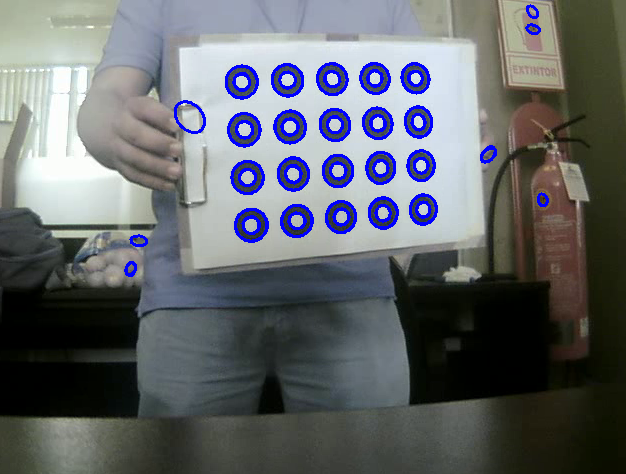
\includegraphics[width=2.5in]{_img/img_results_p1.png}
\caption{Results using pipeline 1.}
\end{figure}
%
\begin{figure}[H]
\centering
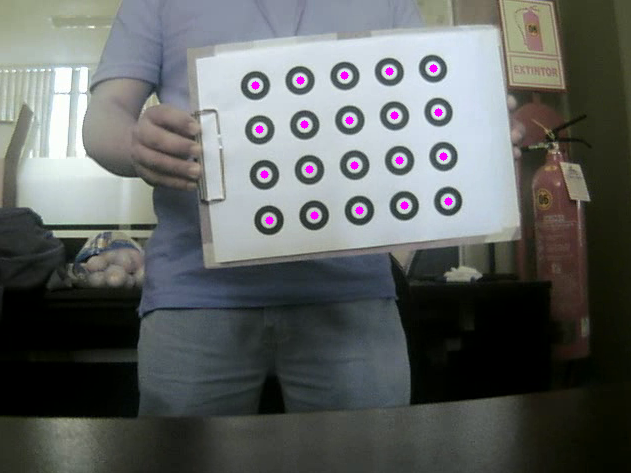
\includegraphics[width=2.5in]{_img/img_results_p2.png}
\caption{Results using pipeline 2.}
\end{figure}
%
\section{Conclusions and Future improvements}
The main issue in both pipeline implementations is that we are using just global information from each frame. This gives some acceptable results, but in cases where there is quite some changes in ilumination, the pipeline may break. In these situations, we could use the fact that the pattern is moving, as well as the fact that the pattern is fixed and the resulting centers should be in a grid like pattern in some way.
\\
\\
We plan on using object tracking, by using an initial estimation of the circles. To get an initial estimation we plan on isolating a region of interest manually, and then track the initial estimation using optical flow or some other techniques, as shown in the following figure.
\\
\begin{figure}[H]
\centering
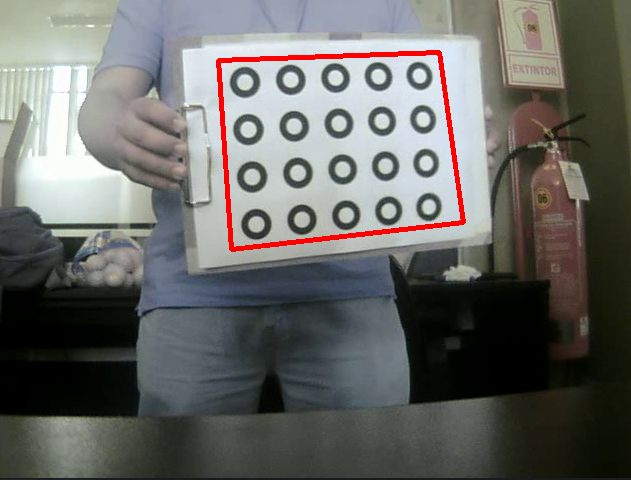
\includegraphics[width=2.5in]{_img/img_results_fut_1.png}
\caption{Initial estimation.}
\end{figure}
%
We plan on also use some fitting method to ensure that we can remove outliers from the grid pattern.

\IEEEtriggeratref{8}

% references section
\begin{thebibliography}{1}

\bibitem{OpenCV}
  Bradski, G. \\
  \textit{OpenCV library.} - 2000
\\
\bibitem{CameraCalibration1}
  Zhengyou Zhang \\
  \textit{A Flexible New Technique for Camera Calibration.} - 2000
\\
\bibitem{IntegralImageThresholding}
  Derek Bradley, Gerhard Roth \\
  \textit{Adaptive Thresholding Using the Integral Image.} - 2011


\end{thebibliography}


\end{document}


